\documentclass{article}

\usepackage[margin=1.5in]{geometry}
\usepackage{graphicx}
\usepackage{booktabs}

\title{A video indexer for searching macroscopic features with deep learning}
\author{Gary Liu (jl25)}
\date{\today}

\begin{document}

\maketitle

\section{Introduction}

Deep learning has been leveraged in performing many image and video processing tasks. Computer vision problems with images, such as object recognition, optical character recognition (OCR), face and emotion recognition, have reached state-of-the-art performance due to the adoption of deep learning. Video-related tasks including action recognition, video object segmentation, video classification, and video generation have also experienced a boost by modern deep learning approaches. Since video is essentially a time series of images, the success of video processing relies heavily on the success of image processing. In fact, it is common practice to treat video data on a per-frame basis, extract spatial features from each frame, and then analyze the temporal behavior (Chen et al, 2010; Le et al, 2011). 

Translation between text and multimedia has attracted much effort from the industry. Microsoft Cognitive Service implements a comprehensive image-processing service and employed it into its real-time per-frame video annotation service. On the other hand, indexing video content by text remains a largely unresolved problem. The text description, or keyword, should describe the entirety of the frame instead of focusing on a specific region of object (which should be addressed by object recognition and segmentation). Potential application is enhancing video searching experience on video sharing platforms by providing content-based searching in addition to searching with caption and labels. People could also find it convenient to locate segments with certain content characteristics in long videos. 

This problem is mostly related to image retrieval, where the candidate video serves as the image database. One approach to image retrieval is automatic image annotation, the process of mapping an image to a caption description or a set of keywords. One drawback of automatic image annotation applied on video indexing is that search relies on the metadata of the image, so the quality of the annotation is important. If the keyword well describes the image but not exactly included in the annotation, search will fail. Another drawback is that simple experiment on Microsoft or Google API shows that their implementation of annotation is largely based on object recognition, and largely produces objects as tags. This could leave out tags that describes the image as a whole. 

Another approach to image retrieval is content-based image retrieval (CBIR), which searches for images in large collection. CBIR directly deals with the pixel content of the image rather than metadata, but its success relies on finding good example images. This could induce problem with searching for objects in images, but could be less problematic when trying to grasp the macroscopic feature of images. In this project we take a CBIR-fashion approach. 

\section{Method}

We break down the task into three steps. First, design and implement a model that binary classifies images. Then, find positive and negative (with respect to the keyword) example images as training data and train the binary classifier. Finally, parse the video into frames at a fixed interval and let the classifier predict whether each frame matches the keyword or not. 

Our performance metric is defined in terms of precision and recall, since we intend to recognize as many matching frames as possible while attempting to reduce the rate of false alarms. For this pilot project, we will look into the classification result to see if the recognized frames make sense (have reasonable relevance with the keyword, and if matching frames are correctly picked out by the classifier. 

It is common practice to draw from existing pre-trained model with state-of-the-art performance (Girshick et al, 2015). The VGG-16 model is shown to have extraordinary performance on the ImageNet dataset, and generalizes well to other datasets (Simonyan, 2014). We leverage the trained weights in the VGG-16 architecture and use the features before the fully connected layers (called the bottleneck features) as representation of images. Figure \ref{fig:vgg-16} depicts the schematic architecture of VGG-16 model. 

\begin{figure}[h]
	\label{fig:vgg-16}
	\centering
	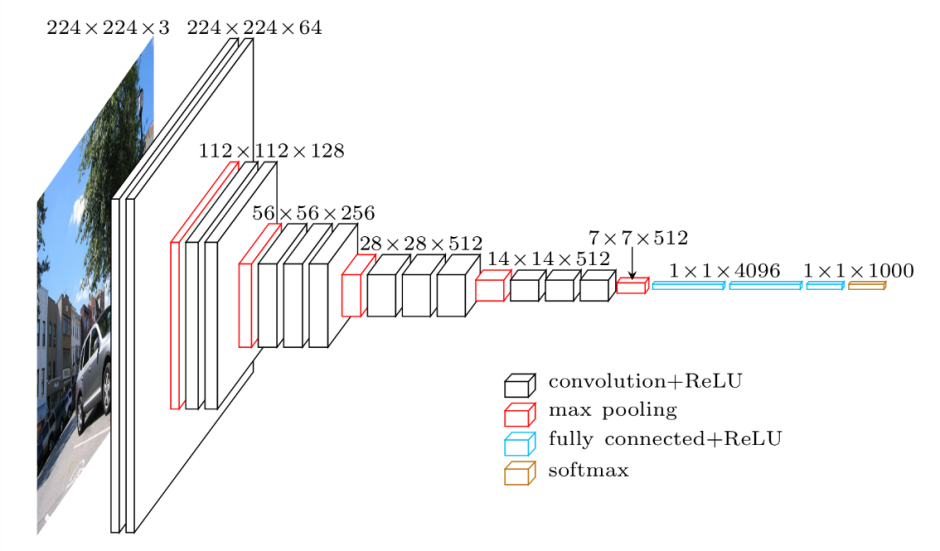
\includegraphics[scale=0.4]{image/vgg16.png}
	\caption{Architecture of VGG-16 deep convolutional neural network for image classification. Image credit to https://blog.heuritech.com/2016/02/29/a-brief-report-of-the-heuritech-deep-learning-meetup-5/}
\end{figure}

\begin{figure}[h]
	\label{fig:model}
	\centering
	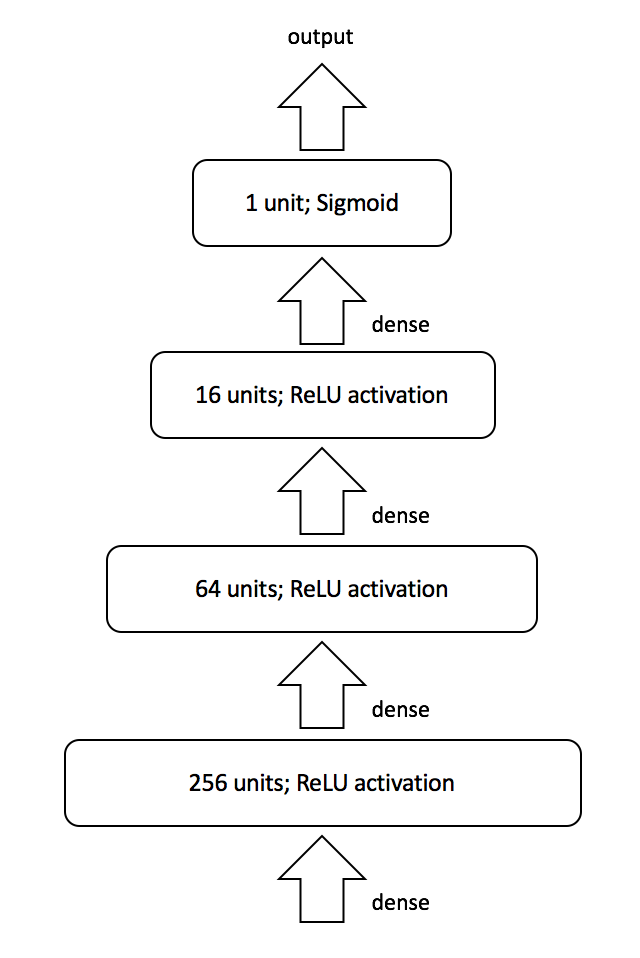
\includegraphics[scale=0.6]{image/dense.png}
	\caption{Additional network placed on top of VGG-16 and predicts image relevance to keyword. To be trained with VGG-16 bottleneck feature. Each dense layer has a dropout rate of 0.5. }
\end{figure}

With the transformed representation of images, we train an additional fully-connected network on top of the VGG-16 model. This network is depicted in Figure \ref{fig:model}. 

We explore the possibility of learning a good binary classifier with data retrieved from Google image search. More specifically, we search by the keyword and use the top results as examples of the keyword. 

\section{Result}

For each keyword of the search, 100 images are retrieved from Google Image searched with this keyword, labeled as positive examples; 100 images are retrieved by searching either the antonym of the keyword or the qualifier "not" concatenated with the keyword, depending on which gives a better match, and labeled as negative examples; 100 random images are also retrieved to be used as negative examples. 

For the candidate video, we use the documentary video \textit{Timescapes}, which features scenes that are easy to describe macroscopically. We choose a frame sampling interval of 1 second. 

Table \ref{tab:result} shows that searches with various keywords successfully recognize corresponding frames. 

\begin{table}[t]
	\label{tab:result}
    \centering
    \caption{Search keywords and corresponding exemplary frames recognized as matching the keywords in the video. Image captured from \textit{Timescapes}. }
    \begin{tabular}{c c c c}
    	\toprule
    	Keyword & & Recognized frames & \\
    	\midrule
    	arid
    		& 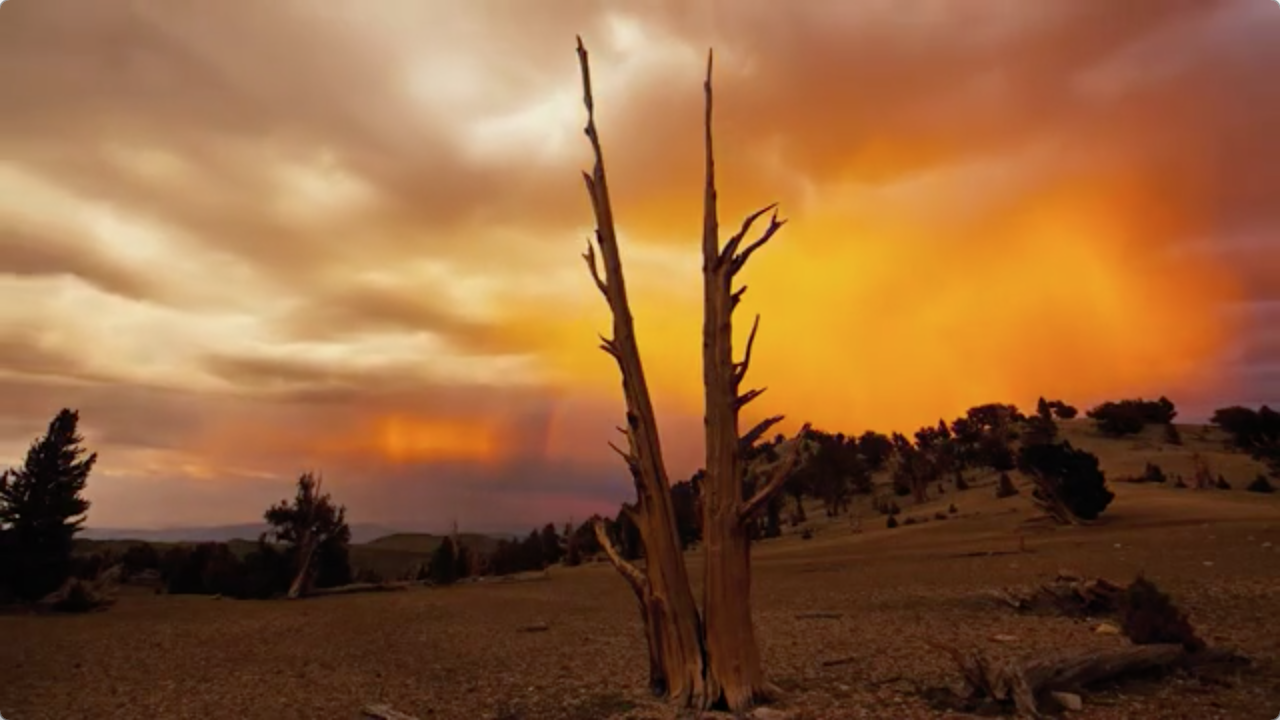
\includegraphics[width=4cm,height=3cm]{image/arid-1.png}
    		& 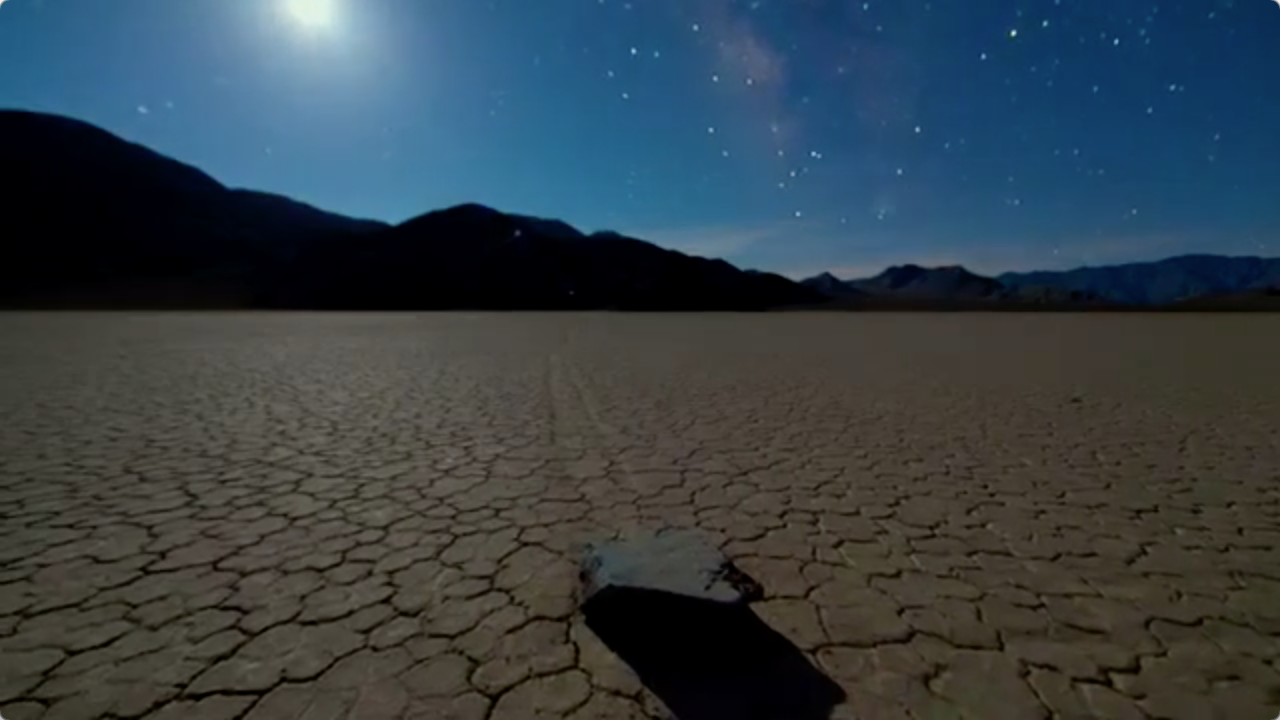
\includegraphics[width=4cm,height=3cm]{image/arid-2.png}
    		& 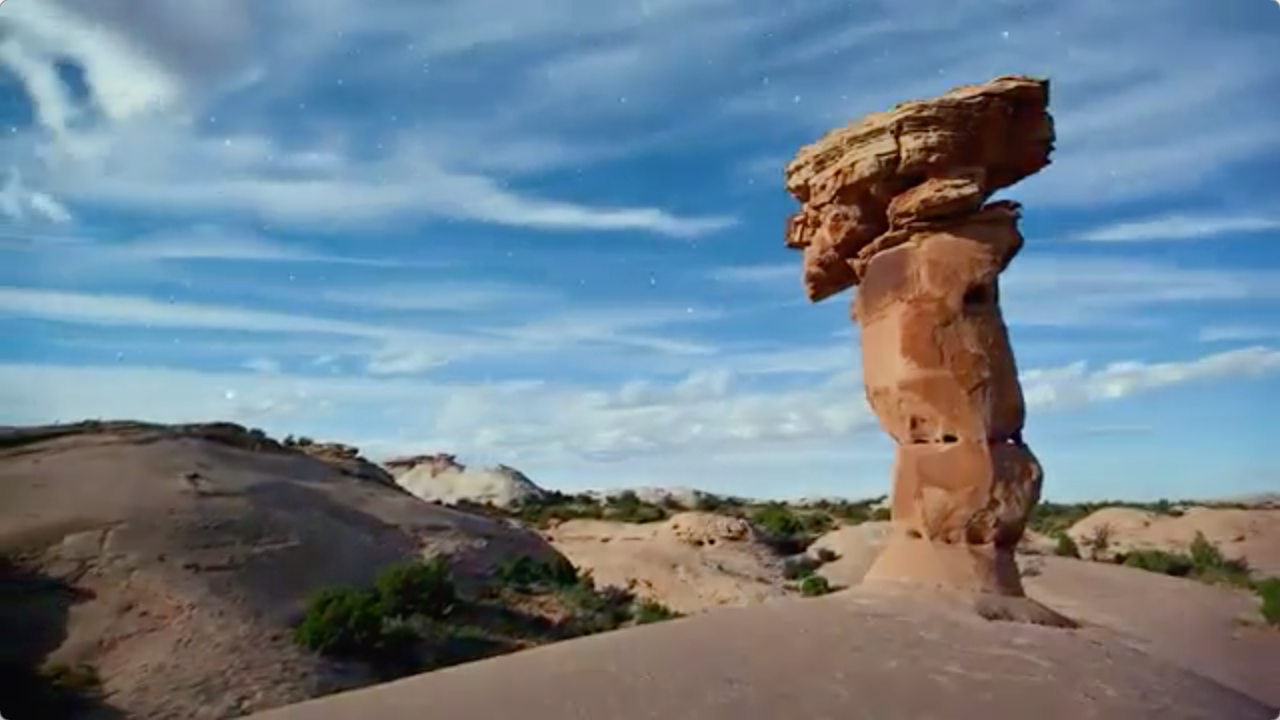
\includegraphics[width=4cm,height=3cm]{image/arid-3.png}
    		\\
    	\midrule
    	crowded
    		& 
\includegraphics[width=4cm,height=3cm]{image/crowded-1.png}
    		& 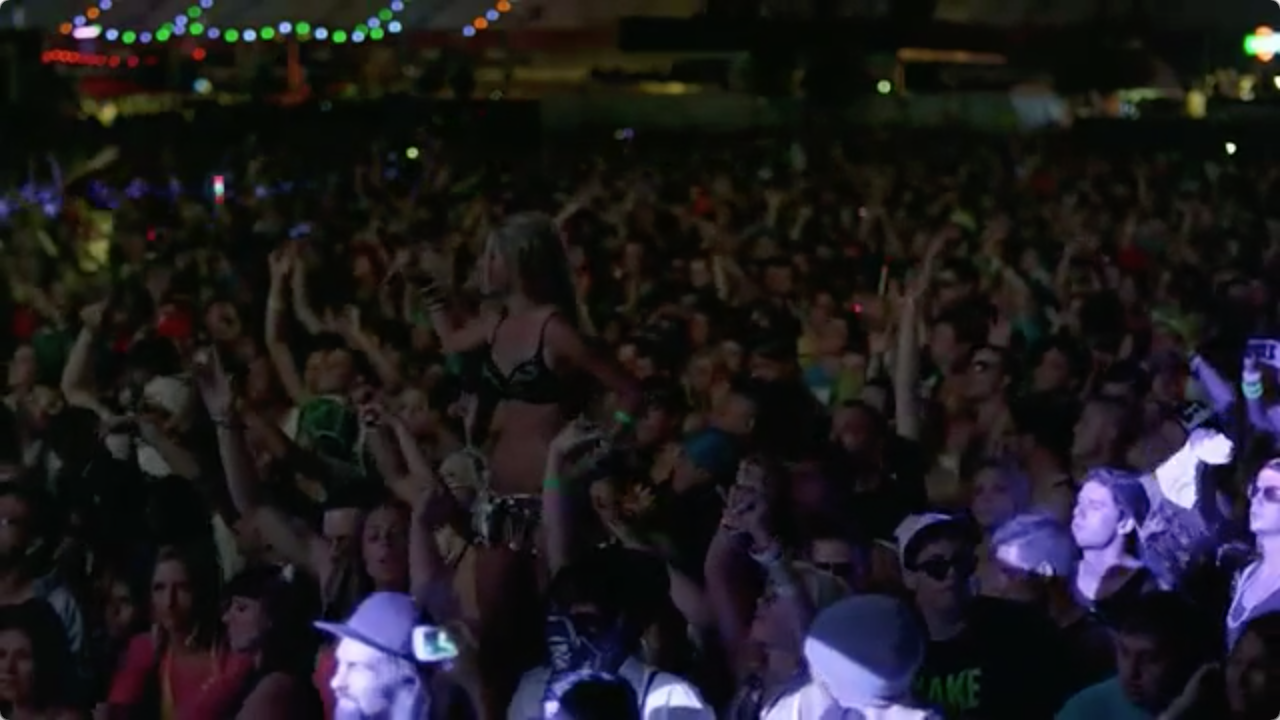
\includegraphics[width=4cm,height=3cm]{image/crowded-2.png}
    		& 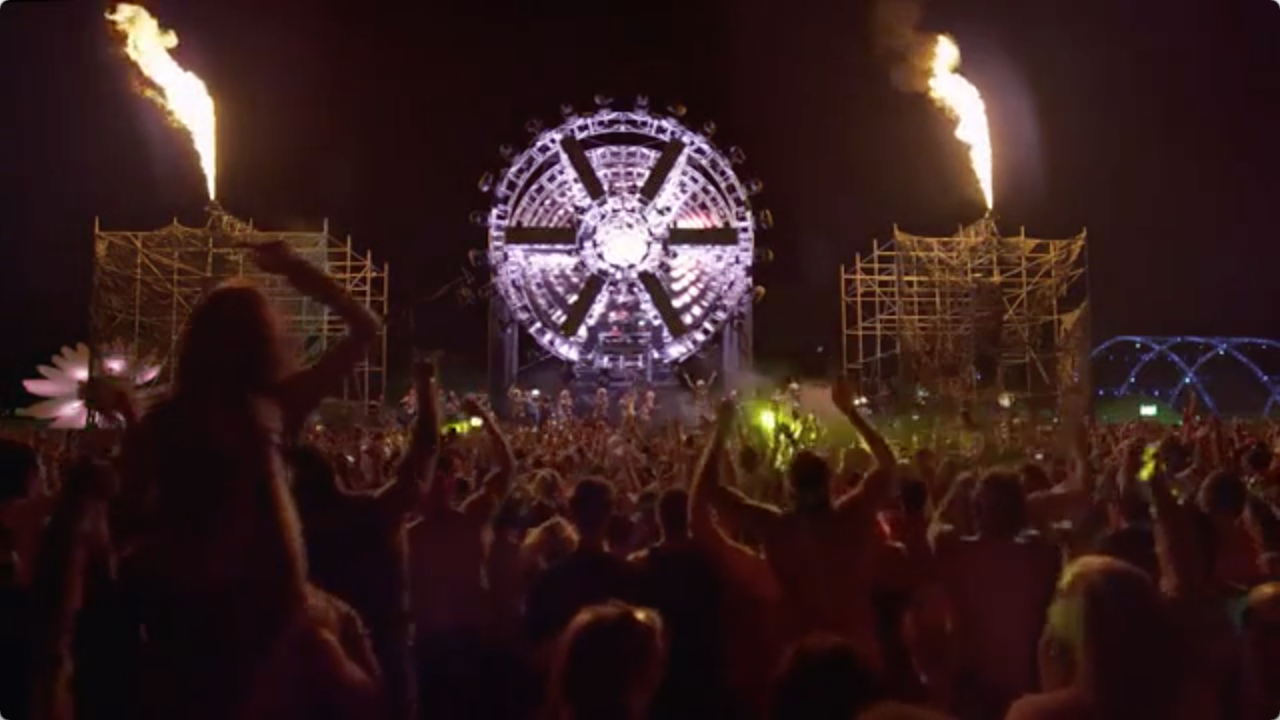
\includegraphics[width=4cm,height=3cm]{image/crowded-3.png}
    		\\
    	\midrule
    	mountainous
    		& 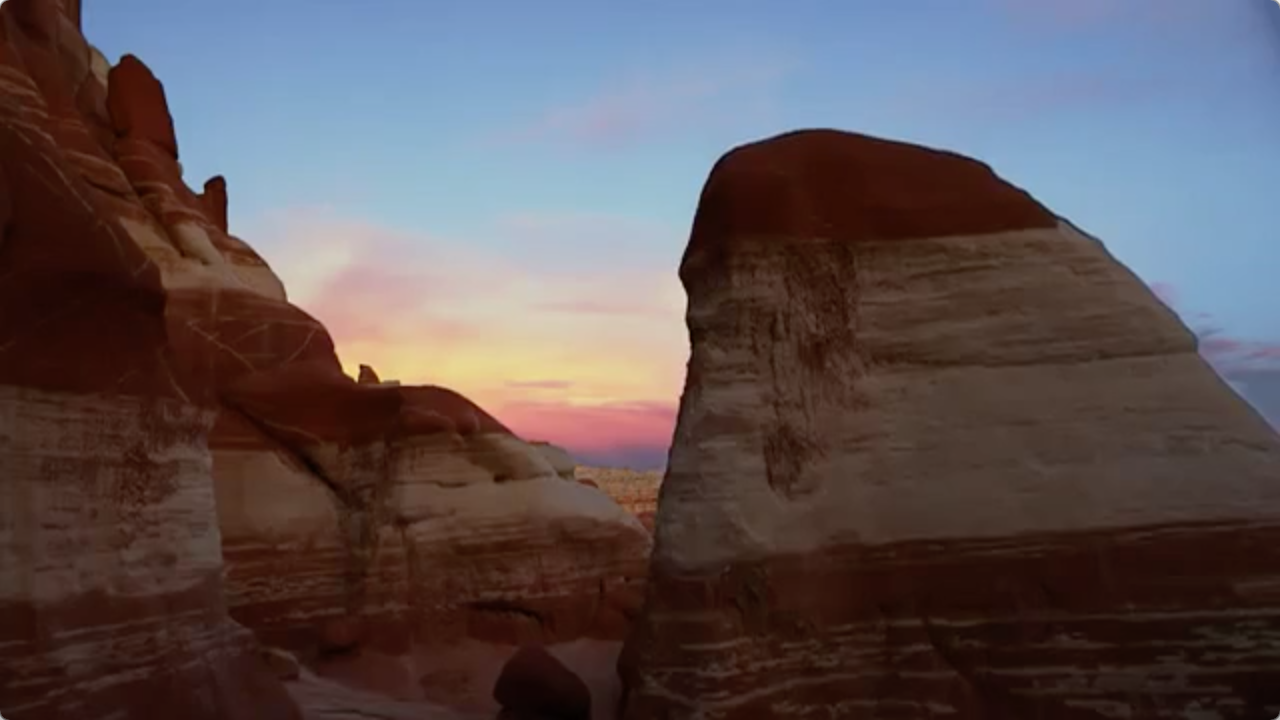
\includegraphics[width=4cm,height=3cm]{image/mountainous-1.png}
    		& 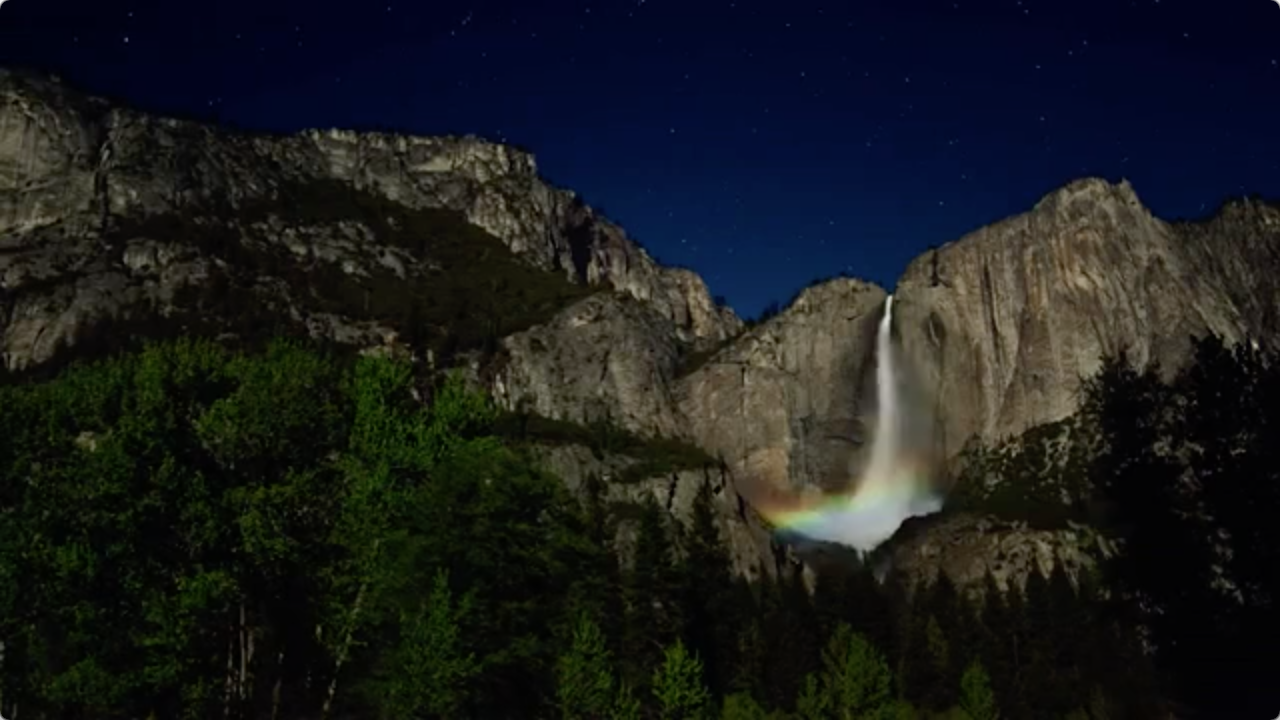
\includegraphics[width=4cm,height=3cm]{image/mountainous-2.png}
    		& 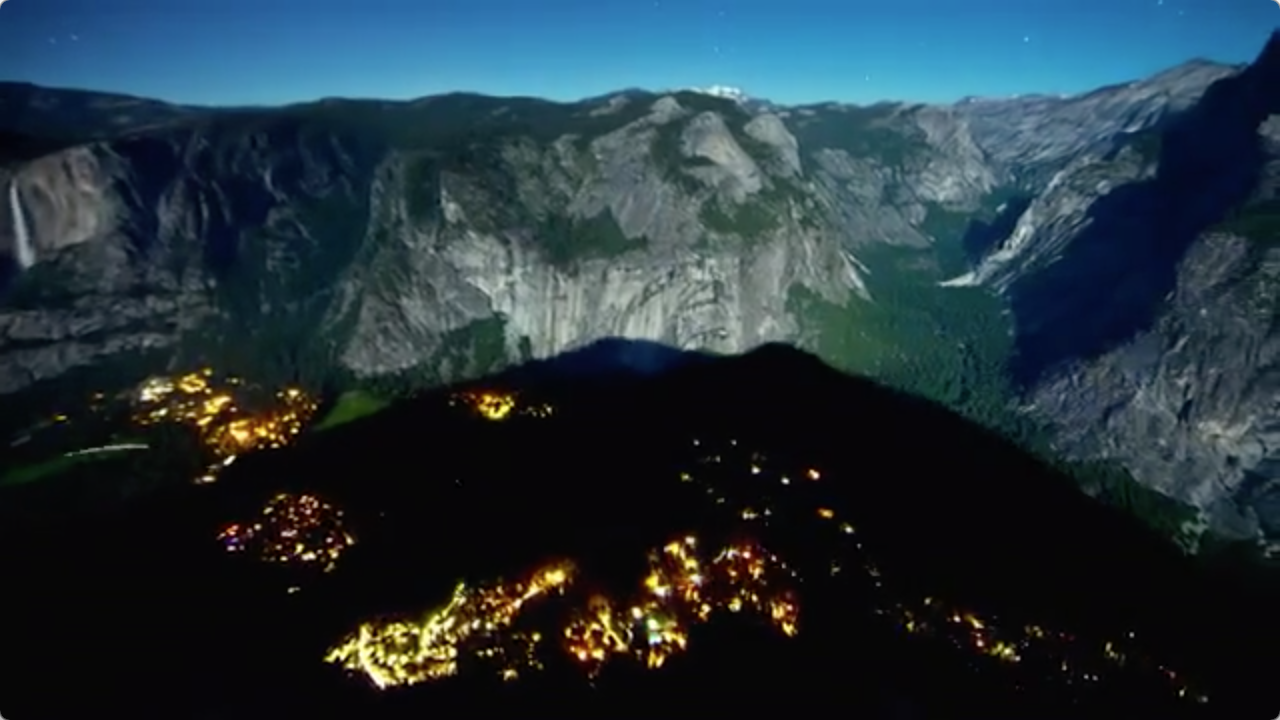
\includegraphics[width=4cm,height=3cm]{image/mountainous-3.png}
    		\\
    	\midrule
    	starry
    		& 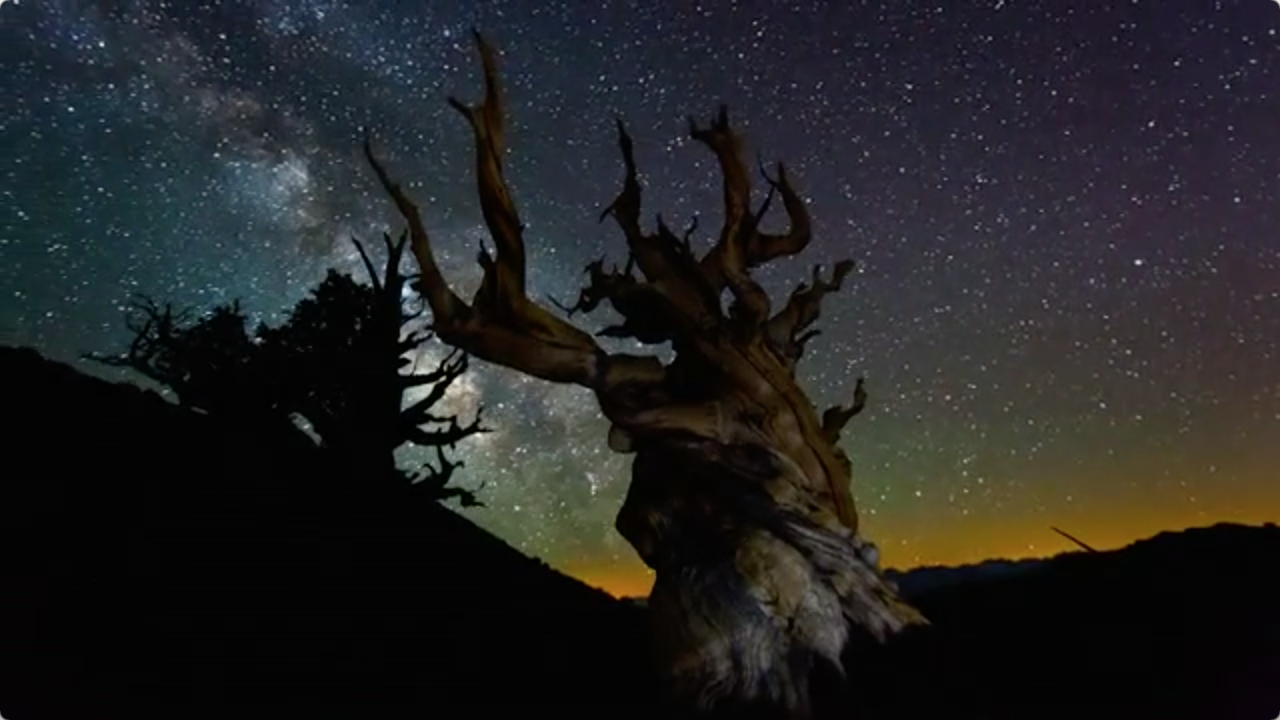
\includegraphics[width=4cm,height=3cm]{image/starry-1.png}
    		& 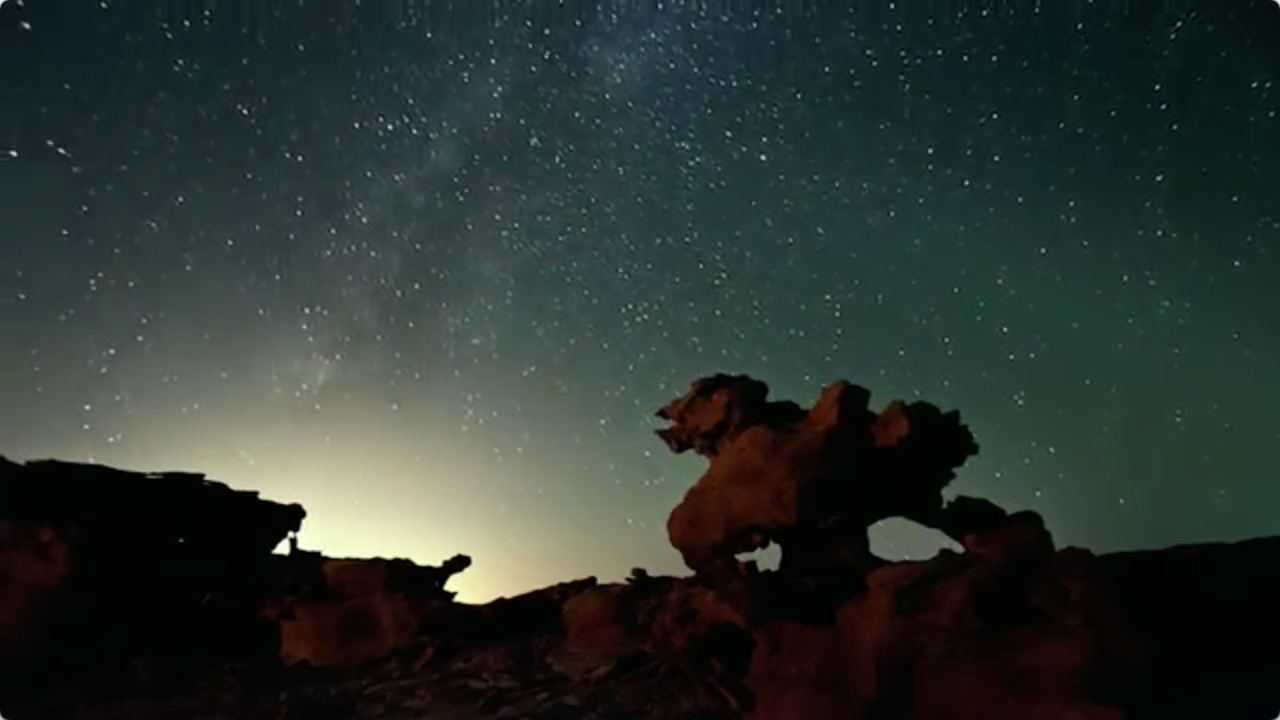
\includegraphics[width=4cm,height=3cm]{image/starry-2.png}
    		& 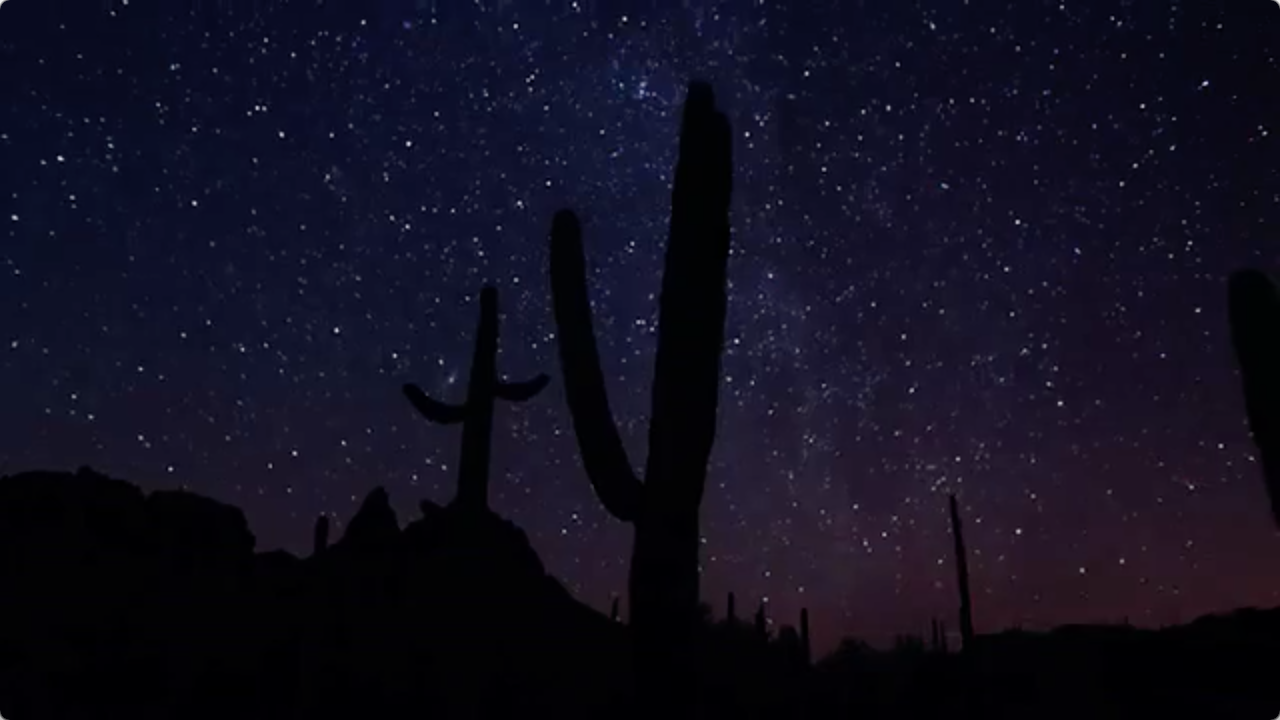
\includegraphics[width=4cm,height=3cm]{image/starry-3.png}
    		\\
    	\bottomrule
    \end{tabular}
\end{table}

Despite the fact that this model recognizes most of the matching frames (high recall rate), the result also includes many irrelevant frames (low precision rate). In videos that we search through, positive frames should occur much less frequent than negative frames, but our selection of training data has nearly equivalent amount of positive and negative examples. Moreover, negative examples should be characterized by "cannot be described by the keyword", not "can be described by the antonym of the keyword". The latter will introduce a large confusion region in the middle of the two classes. This analysis motivates us to collect more random images to use as negative examples in the training stage. 

One observation is that some negative examples retrieved from the image search engine are more likely to be a positive example (this is due to the fact that search engines may encounter problem generating counter-examples). With such noise in the training data, the model can still reach a near-zero training error, so we speculate that some overfitting is present. 

%\section{Conclusion}

\section{Note}

This is the final project of CS 598 PS. A team of two students was formed to work on this project, but I have not been able to contact my teammate since the proposal was due, so I worked out everything of this project by myself. Please be considerate when grading it. 

\section{References}

K. Simonyan, A. Zisserman. 2014. Very Deep Convolutional Networks for Large-Scale Image Recognition. arXiv:1409.1556 [cs.CV]

B. Chen, J. A. Ting, B. Marlin, and N. de Freitas. Deep learning of invariant spatio-temporal features from video. In NIPS Deep Learning and Unsupervised Feature Learning Workshop, 2010.

Q. V. Le, W. Y. Zou, S. Y. Yeung, and A. Y. Ng. 2011. Learning hierarchical invariant spatio-temporal features for action recognition with independent subspace analysis. In Proceedings of the 2011 IEEE Conference on Computer Vision and Pattern Recognition (CVPR '11). IEEE Computer Society, Washington, DC, USA, 3361-3368. DOI=http://dx.doi.org/10.1109/CVPR.2011.5995496

\end{document}
